\documentclass[12pt]{article}
\usepackage[utf8]{inputenc}
\usepackage[colorlinks]{hyperref}
\usepackage{cite}
\usepackage{graphicx}
\usepackage{float}

\title{Project Checkpoint: CSE 6730 Project 1}
\author{Chris Dunlap, Allen Koh, Matt May}
\date{February 2016}

\begin{document}

\begin{titlepage}
\maketitle
\thispagestyle{empty}
\end{titlepage}

\section{Problem Statement}
\label{sec:problem}

The efficient evacuation of physical structures is an important problem with a
long history of multi-disciplinary study \cite{zheng2009modeling}. For this
study, we focus specifically on the problem of efficiently evacuating the
area around Bobby Dodd Stadium in Atlanta, GA. Bobby Dodd Stadium, the home of
the the NCAA Division-I Georgia Tech Yellow Jackets football team, has a
seating capacity of 55,000 individuals.

\begin{figure}[H]
  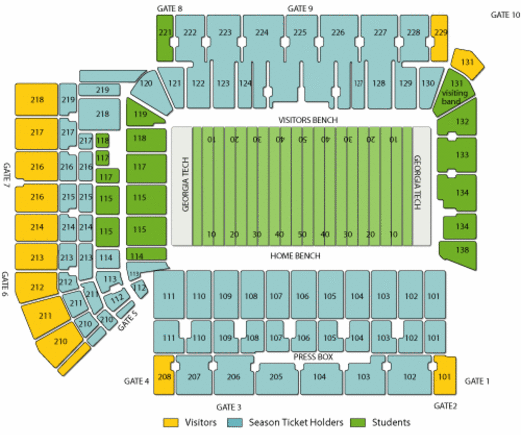
\includegraphics[width=\linewidth,natwidth=521,natheight=435]{stadium_diagram_updated.png}
  \caption{Bobby Stadium Stadium seating chart.}
  \label{fig:polygon}
\end{figure}

Our primary objective in this study is to minimize the pedestrian evacuation
time of the stadium and its surrounding area as attendees leave the area
following a home football game. We do this by taking a parametric approach, in
which we explore the effects of road closures, strategically placed guidance
symbols (i.e., signs), and the ``takeover" of certain intersections by law
enforcement in promoting an optimal result.

For purposes of this study, we define the system under investigation (SUI) as a
rectangular polygon (Fig. \ref{fig:polygon}) surrounding the stadium. To be clear,
the SUI is defined as the area inside the polygon but outside the stadium. As
pedestrians exit the stadium, they enter the SUI, and as the cross the boundary
of the polygon, they exit it.

\begin{figure}[H]
  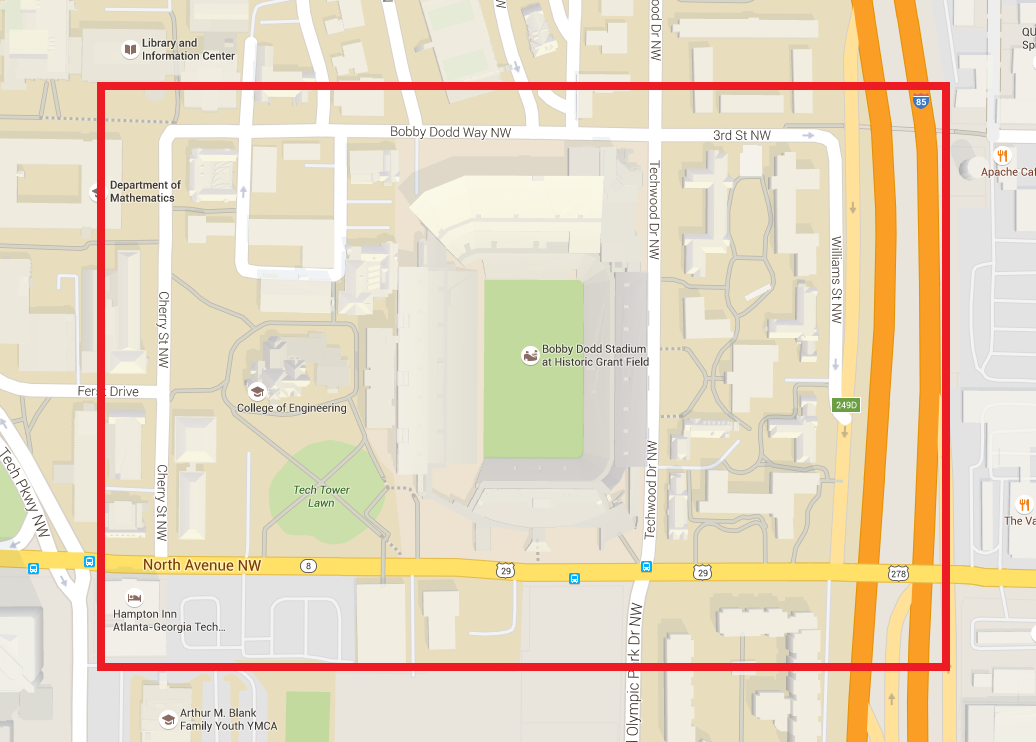
\includegraphics[width=\linewidth,natwidth=1036,natheight=742]{cropped_map.png}
  \caption{The system under investigation.}
  \label{fig:polygon}
\end{figure}

The stadium has 10 ``gates," which serve as ingress (pre-game) and egress
(post-game) sites. These serve as the entry points to our simulation. As
pedestrians enter the SUI, they are assigned a destination and then proceed
to their destination by way of pedestrian walking paths (i.e., sidewalks).

\section{Related Work}
\label{sec:literature}

A variety of techniques have been used to model pedestrian movement. Cellular
automata, lattice gas, social force, fluid-dynamic, agent-based, game-theoretic,
and animal experimention-based approaches have been used
\cite{zheng2009modeling}. As noted by Zheng, Zhong, and Liu
\cite{zheng2009modeling}, models often encounter or attempt to model several
common phenomenoma: clogging, side-stepping, lane formation, and herding
behavior, among them.

These phenomena manifest themselves in different ways and at different
magnitudes depending on the system being modeled. In one of the early
explorations of 2D cellular automata for simulating traffic flow in the related
domain of vehicular traffic simulation, Biham and Middleton \cite{biham1992self}
note the presence of a sharp
\textit{jamming transition} in which all cars in the simulation transition from
moving at maximal speed to being stuck. Similar effects were noted in
simulations of bi-directional pedestrian movement, with Weifeng, Lizhong, and
Weicheng \cite{weifeng2003simulation} finding that as total pedestrian density
increases, a critical value is reached at which the system transitions into a
jammed state where only a few pedestrians are able to proceed.

In a slightly different take on the problem, Okazaki and Matsushita
\cite{okazaki1993study} modeled pedestrian evacuation using Coulomb's Law, with
actors magnetically moving toward their goals and away from obstacles that would
lead to collisions. In another application of equations of natural phenomena,
Helbing \cite{helbing1998fluid} derived fluid dynamic equations for explaining
the movement of pedestrian crowds, observing phenomena such as the development
of lanes, jamming, and crossing. Helbing \cite{helbing2000simulating} further
notes an explicit ``faster-is-slower" effect, in which attempting to move faster
results in a smaller average speed of leaving at high pedestrian density in
evacuation scenarios.

In a more recent study, Helbing et al. \cite{helbing2005self} use a
``social force" model, which states that pedestrians operate in some sense
automatically when reacting to obstacles and other pedestrians, applying
strategies that have been learned to be most effective over time. Several
suggestions are made to alleviate the three most common problems in pedestrian
crowds: counterflows, bottlenecks, and intersecting flows. The presence of
strategically placed obstacles are found to actually reduce these negative
phenomena, leading to improved flow.

Building on previous cellular automata-based models, Burstedde et al.
\cite{burstedde2001simulation} introduce a \textit{floor field}, a secondary
grid of cells which underlies the main grid and acts as a substitute for
pedestrian intelligence. These fields can be either static or dynamic, and are
capable of promoting the avoidance of jams, as well as simulating attractive
effects, in which pedestrians are more likely to follow in the paths of
pedestrians ahead of them.

Taking a more algorithmic approach, Fang et al. \cite{fang2011hierarchical} have
designed a modified ant colony optimization (ACO) algorithm for optimizing
pedestrian evacuation, seeking to minimize evacuation time, evacuation distance,
and congestion. Kemloh Wagoum, Seyfried, and Holl \cite{kemloh2012modeling}
utilize an observation principle approach in modeling pedestrian evacuation,
in which pedestrians first observe their environment and then make a final
decision on strategy based on obtained data.

There are several takeaways from the literature described above that have
potential applicability to the model at hand. First, on the topic of modeling
pedestrian walkways, several papers focused on either a single passageway,
enclosed areas with obstacles (walls, pillars, etc.), or evacuation from a
room with a single doorway. However, modeling walkways as a directed graph
\cite{fang2011hierarchical} seems feasible given the problem at hand, where
there are multiple pathways one can take to get to a single destination. In
papers where cellular automata was utilized, the median size of each cell on the
walkway was 0.4m\textsuperscript{2}
\cite{blue2001cellular,burstedde2001simulation,weifeng2003simulation}.

Second, on the topic of pedestrian modeling, multiple walking speed techniques
were used, ranging from a constant speed of 1 m/s \cite{weifeng2003simulation}
or 1.3 m/s \cite{burstedde2001simulation}, to using a distribution resembling a
step function \cite{blue2001cellular} or a Normal distribution
\cite{klupfel2005models}. In either distribution, the median walking speed was
also approximately 1.3 m/s. For reaction to stimuli, 0.3 seconds was utilized
\cite{burstedde2001simulation}, which was one time step in that particular
simulation. Incorporation of opportunistic side-stepping was done
\cite{blue2001cellular}, in addition to using least-cost algorithms for
establishing the path a pedestrian would like to take
\cite{fang2011hierarchical}. In the context of cellular automata, analyzing a
given pedestrian's cell's neighbors in either a 4-connected
\cite{weifeng2003simulation} or 8-connected fashion
\cite{burstedde2001simulation} to decide in which direction the pedestrian would
like to walk for the next time step was utilized. This, coupled with a dynamic
floor field \cite{burstedde2001simulation} to factor in long-distance forces,
could be utilized.

Finally, simulation execution practices were also gleaned. Care must be taken
to do parallel-based updating to avoid sequential updating from interfering with
underlying model execution \cite{blue2001cellular}. The practice of using
a deterministic model running with randomized initial conditions has precedent
\cite{biham1992self}. Finally, to achieve statistical significance, 20 runs per
configuration has been used \cite{blue2001cellular}.

\section{Conceptual Model}
For our simulation, we utilize a 2-dimensional cellular automata (CA)-based
approach. We construct a discrete time-stepped model, in which the simulation
clock advances by a fixed interval every time step. We utilize a stochastic
(probabilistic) approach, in which the output of each individual simulation
run is a random variable. Thus, multiple simulation runs will be performed and
statistical analysis will be used to provide confidence levels in our results.

\subsection{Inputs}
The primary input to our simulation model is a stream of football game attendees
(i.e., pedestrians) exiting Bobby Dodd Stadium following a home football game.
For purposes of modeling this input stream, we assume pedestrian interarrival
time at the stadium gate boundary is a homogenous stochastic process that
follows a \textit{TODO: insert} distribution. As pedestrians arrive at the gate
boundary, they enter the SUI.

In addition, we select each pedestrian's target destination and walking
speed at random. For selecting a target destination, we utilize \textit{TODO: Allen?}
For determining a walking speed for each pedestrian, we sample from a
distribution previously referenced in the literature by Blue and Adler
\cite{blue2001cellular} (5\% fast walkers (4 cells/time step), 90\% standard
(3 cells/time step), 5\% slow (2 cells/time step)).

Pedestrians in our model can be considered a consumer entity class
\textit{Pedestrian} with attributes which will be set and updated during the
course of our simulation. Table \ref{table:ped} provides an overview of the
attributes of the \textit{Pedestrian} class.

\def\arraystretch{1.5}
\begin{table}[hb!]
  \centering
    \begin{tabular}{p{0.2\linewidth}p{0.6\linewidth}}
     \hline
     Attribute & Description \\
     \hline
     % StartTime & Simulation clock value when the pedestrian enters the
                 % simulation. \\
     % Duration & Total duration of simulation time in which the pedestrian
                % exists in the simulation. \\
     DestinationID  & NodeID of the final destination of the pedestrian. \\
     Speed          & Walking speed, formulated in grid cells traversed per
                      time step. \\
     NodeID         & Location of the pedestrian in the simulation, specified
                      by a unique node identifier (NodeID). \\
     EgressComplete & A binary value. This value is 0 when the pedestrian has
                      not yet egressed, and 1 when egress is complete. \\
     \hline
    \end{tabular}
    \caption{Attributes of the \textit{Pedestrian} entity class.}
  \label{table:ped}
\end{table}

New instances of the \textit{Pedestrian} class are created and initialized
as pedestrians exit the stadium.

\subsection{Output}
For each simulation run, when all pedestrians were evacuated from the SUI we
determined the simulation to be complete. As this is a stochastic simulation,
the output results must be interpreted as samples from a random process.

At the conclusion of a series of simulation runs for a given set of parameters,
we compute an average of the total egress duration across all runs from that
series. More formally, the average egress time $E_{avg}$ for $n$ simulation runs
can be represented as:

\begin{equation}
E_{avg} = \frac{1}{n}\sum\limits_{i=1}^n d_i
\end{equation}

where $d_i$ is the total egress duration of the $i$th simulation run. This
output can be considered a derived scalar output variable (DSOV). We then
define the optimal parameter strategy to be the set of parameters $P$ that
give the the minimum value of $E_{avg}$.

\subsection{Content}

\subsubsection{Approach}
Pedestrians exit the stadium from one of four potential exits. To build the
simulation space, we overlay a 2-dimensional cellular automata grid on a map of
the SUI. We model this space as a directed graph, a type of graph in which each
graph edge is replaced by a directed graph edge \cite{west2001introduction}.

As pedestrians exit the stadium, they are probabilistically assigned a
destination node, which can be formulated as a unique node identifier in the
graph. Destinations take one of three possible classes: on-campus housing
(dormitories), parking lots, or the North Avenue Metropolitan Atlanta Rapid
Transit Authority (MARTA) station.

For each node in the graph, we precompute the least-cost path to every possible
desination node. We represent each node as member of a \textit{Node} class, which
has attributes as shown in Table \ref{table:node}.

\def\arraystretch{1.5}
\begin{table}[hb!]
  \centering
    \begin{tabular}{p{0.2\linewidth}p{0.6\linewidth}}
     \hline
     Attribute & Description \\
     \hline
     NodeID      & Unique identifier for the node. \\
     XCoordinate & TODO \\
     YCoordinate & TODO \\
     Paths       & A dictionary (hash map) relating each possible destination
                   to the NodeID of the next node in the shortest path as
                   determined by Dijkstra's algorithm. \\
     \hline
    \end{tabular}
    \caption{Attributes of the \textit{Node} class.}
  \label{table:node}
\end{table}

At each time step, the shortest path approach is selected for every pedestrian
in the path towards their destination. We compute the shortest path between any
source node $N_s$ and destination node $N_d$ using Dijkstra's well-known
algorithm \cite{dijkstra1959note}.

\subsubsection{Parameters}


\subsubsection{Random Numbers}
To model the egress of the stadium, we take a stochastic (probabilistic)
approach. In the context of a computer simulation, this necessitates the use of
a pseudorandom number generator. For this study, we use the simple linear
congruential approach. This generator is given a \textit{seed} value,
and then produces a uniformly distributed pseudorandom number. This value is
then used to sample from a given probability distribution.

\subsection{Assumptions and Simplifications}
Our simulation is simplified by focusing only on \textit{pedestrian} traffic,
avoiding the inclusion of vehicular traffic. In future studies, this could be
included as an enhancement.

\bibliography{template}{}
\bibliographystyle{plain}
\end{document}
